% document
\documentclass[11pt, aspectratio=169, final]{beamer}
\usepackage{adjustbox}
\adjustboxset*{center}
\usepackage{color}
\usepackage{xcolor}
\usepackage{textpos}

\usepackage{amsmath,amsfonts,amsthm} % Math packages
% theme coercion
\usetheme[width=2cm]{Hannover}
\usecolortheme{beaver}
\definecolor{base03}{HTML}{002B36}
\definecolor{base02}{HTML}{073642}
\definecolor{base01}{HTML}{586E75}
\definecolor{base3}{HTML}{FDF6E3}
\definecolor{solarblue}{HTML}{268bd2}
\definecolor{solarmagenta}{HTML}{D33682}
\setbeamercolor*{palette primary}{fg=darkred!60!black, bg=base01}  % title background
\setbeamercolor*{sidebar}{fg=darkred, bg=base03}
\setbeamercolor{frametitle}{bg=base01, fg=base3}
\setbeamercolor{title}{fg=base3}
\setbeamercolor{palette sidebar primary}{fg=base3}  % sidebar subsection
\setbeamercolor{palette sidebar secondary}{fg=base3}  % sidebar section
\setbeamercolor{palette sidebar tertiary}{fg=base3}  % sidebar name
\setbeamercolor{palette sidebar quaternary}{fg=base3}  % sidebar title
\setbeamercolor*{item}{fg=base01}
\setbeamertemplate{itemize items}[default]
\setbeamercovered{transparent}
\setbeamertemplate{navigation symbols}{}

% text
\usepackage[utf8]{inputenc}
\usepackage[T1]{fontenc}
\usepackage{enumerate}
\usepackage{soul}
\sethlcolor{yellow}
\renewcommand<>{\hl}[1]{\only#2{\beameroriginal{\hl}}{#1}}

% code
%\usepackage{minted}
%\definecolor{bg}{rgb}{0.95,0.95,0.95}
%\newminted{python}{fontsize=\scriptsize, numbersep=8pt,	gobble=0, frame=none, bgcolor=bg,	framesep=2mm, frame=leftline}

% quotes
\usepackage[T1]{fontenc}
\usepackage{libertine}
\usepackage{framed}
\newcommand*\openquote{\makebox(25,-22){\scalebox{5}{``}}}
\newcommand*\closequote{\makebox(25,-22){\scalebox{5}{''}}}
\colorlet{shadecolor}{base3}
\makeatletter
\newif\if@right
\def\shadequote{\@righttrue\shadequote@i}
\def\shadequote@i{\begin{snugshade}}
		\def\endshadequote{%
			\if@right\hfill\fi\end{snugshade}}
\@namedef{shadequote*}{\@rightfalse\shadequote@i}
\@namedef{endshadequote*}{\endshadequote}
\makeatother

% graphics
\usepackage{graphicx}
\usepackage{animate}
\usepackage{xmpmulti}

% bibliography
\usepackage[style=verbose,backend=bibtex,bibstyle=numeric,sorting=none]{biblatex}
\bibliography{bib}
\renewcommand\footnoterule{{\color{black} \hrule height 0pt}} % no line above footnotes
\renewcommand{\footnotesize}{\tiny}
\setbeamercolor{bibliography entry author}{fg=black,bg=black}
\setbeamercolor{bibliography entry title}{fg=black,bg=black}
\setbeamercolor{bibliography entry location}{fg=black,bg=black}
\setbeamercolor{bibliography entry note}{fg=black,bg=black}

% http://tex.stackexchange.com/questions/41683/why-is-it-that-coloring-in-soul-in-beamer-is-not-visible
\makeatletter
\newcommand\SoulColor{%
	\let\set@color\beamerorig@set@color
	\let\reset@color\beamerorig@reset@color}
\makeatother
\SoulColor

% logo (not built-in to hannover)
\addtobeamertemplate{headline}{}{%
\begin{textblock*}{\paperwidth}(0.5cm,\textheight-1.75cm)
	
\includegraphics[width=1cm]{logo} % logo of my university
\end{textblock*}}

\title{\textbf{WrightSim}}
\author{Kyle Sunden}
%\subtitle{}

\institute{University of Wisconsin--Madison}
\date{\today}
%\subject{}

\begin{document}
\maketitle

\section{Goals}

\begin{frame}{\textbf{Goals}}
%TODO bulleted list of goals
\end{frame}

\begin{frame}{\textbf{Sample Spectrum}}
\begin{center}
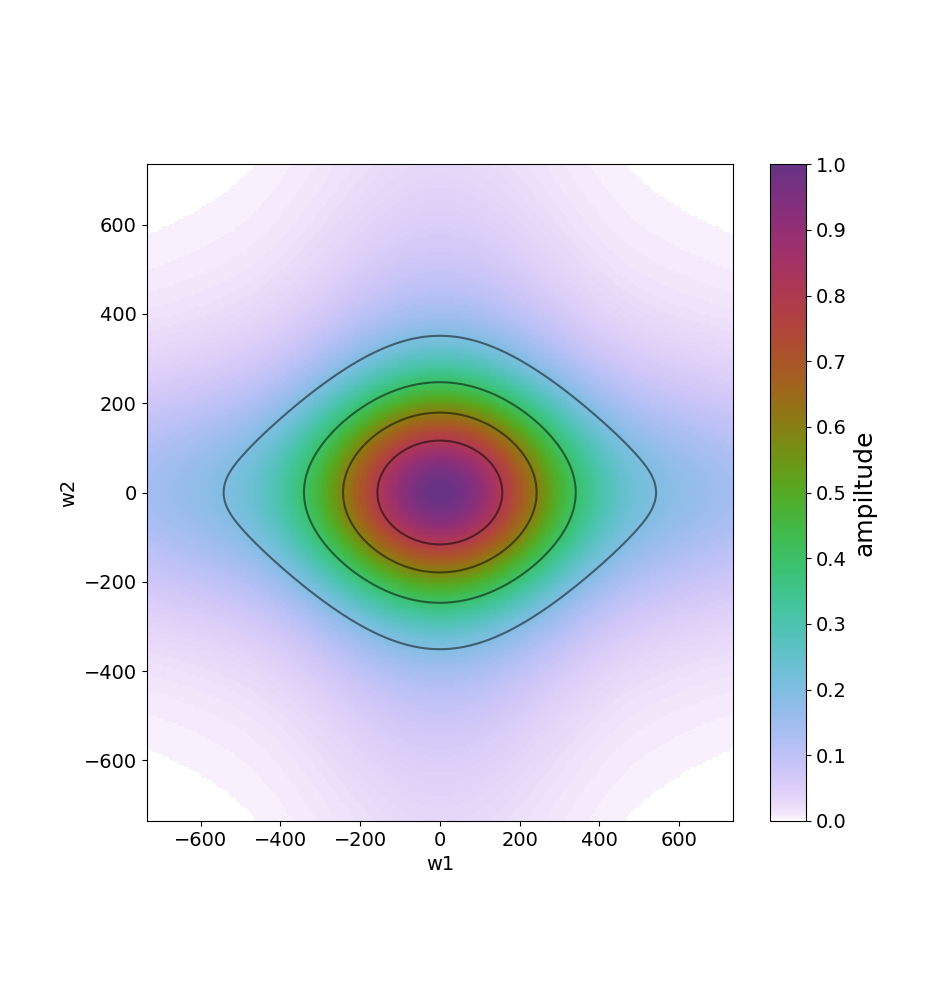
\includegraphics[height=\textheight]{example_spectrum}
\end{center}
\end{frame}


\section{Theory}

\begin{frame}{\textbf{Introduction}}
	Here is some text
%TODO: Text intro
\end{frame}

\begin{frame}{\textbf{Pathways}}
\begin{center}
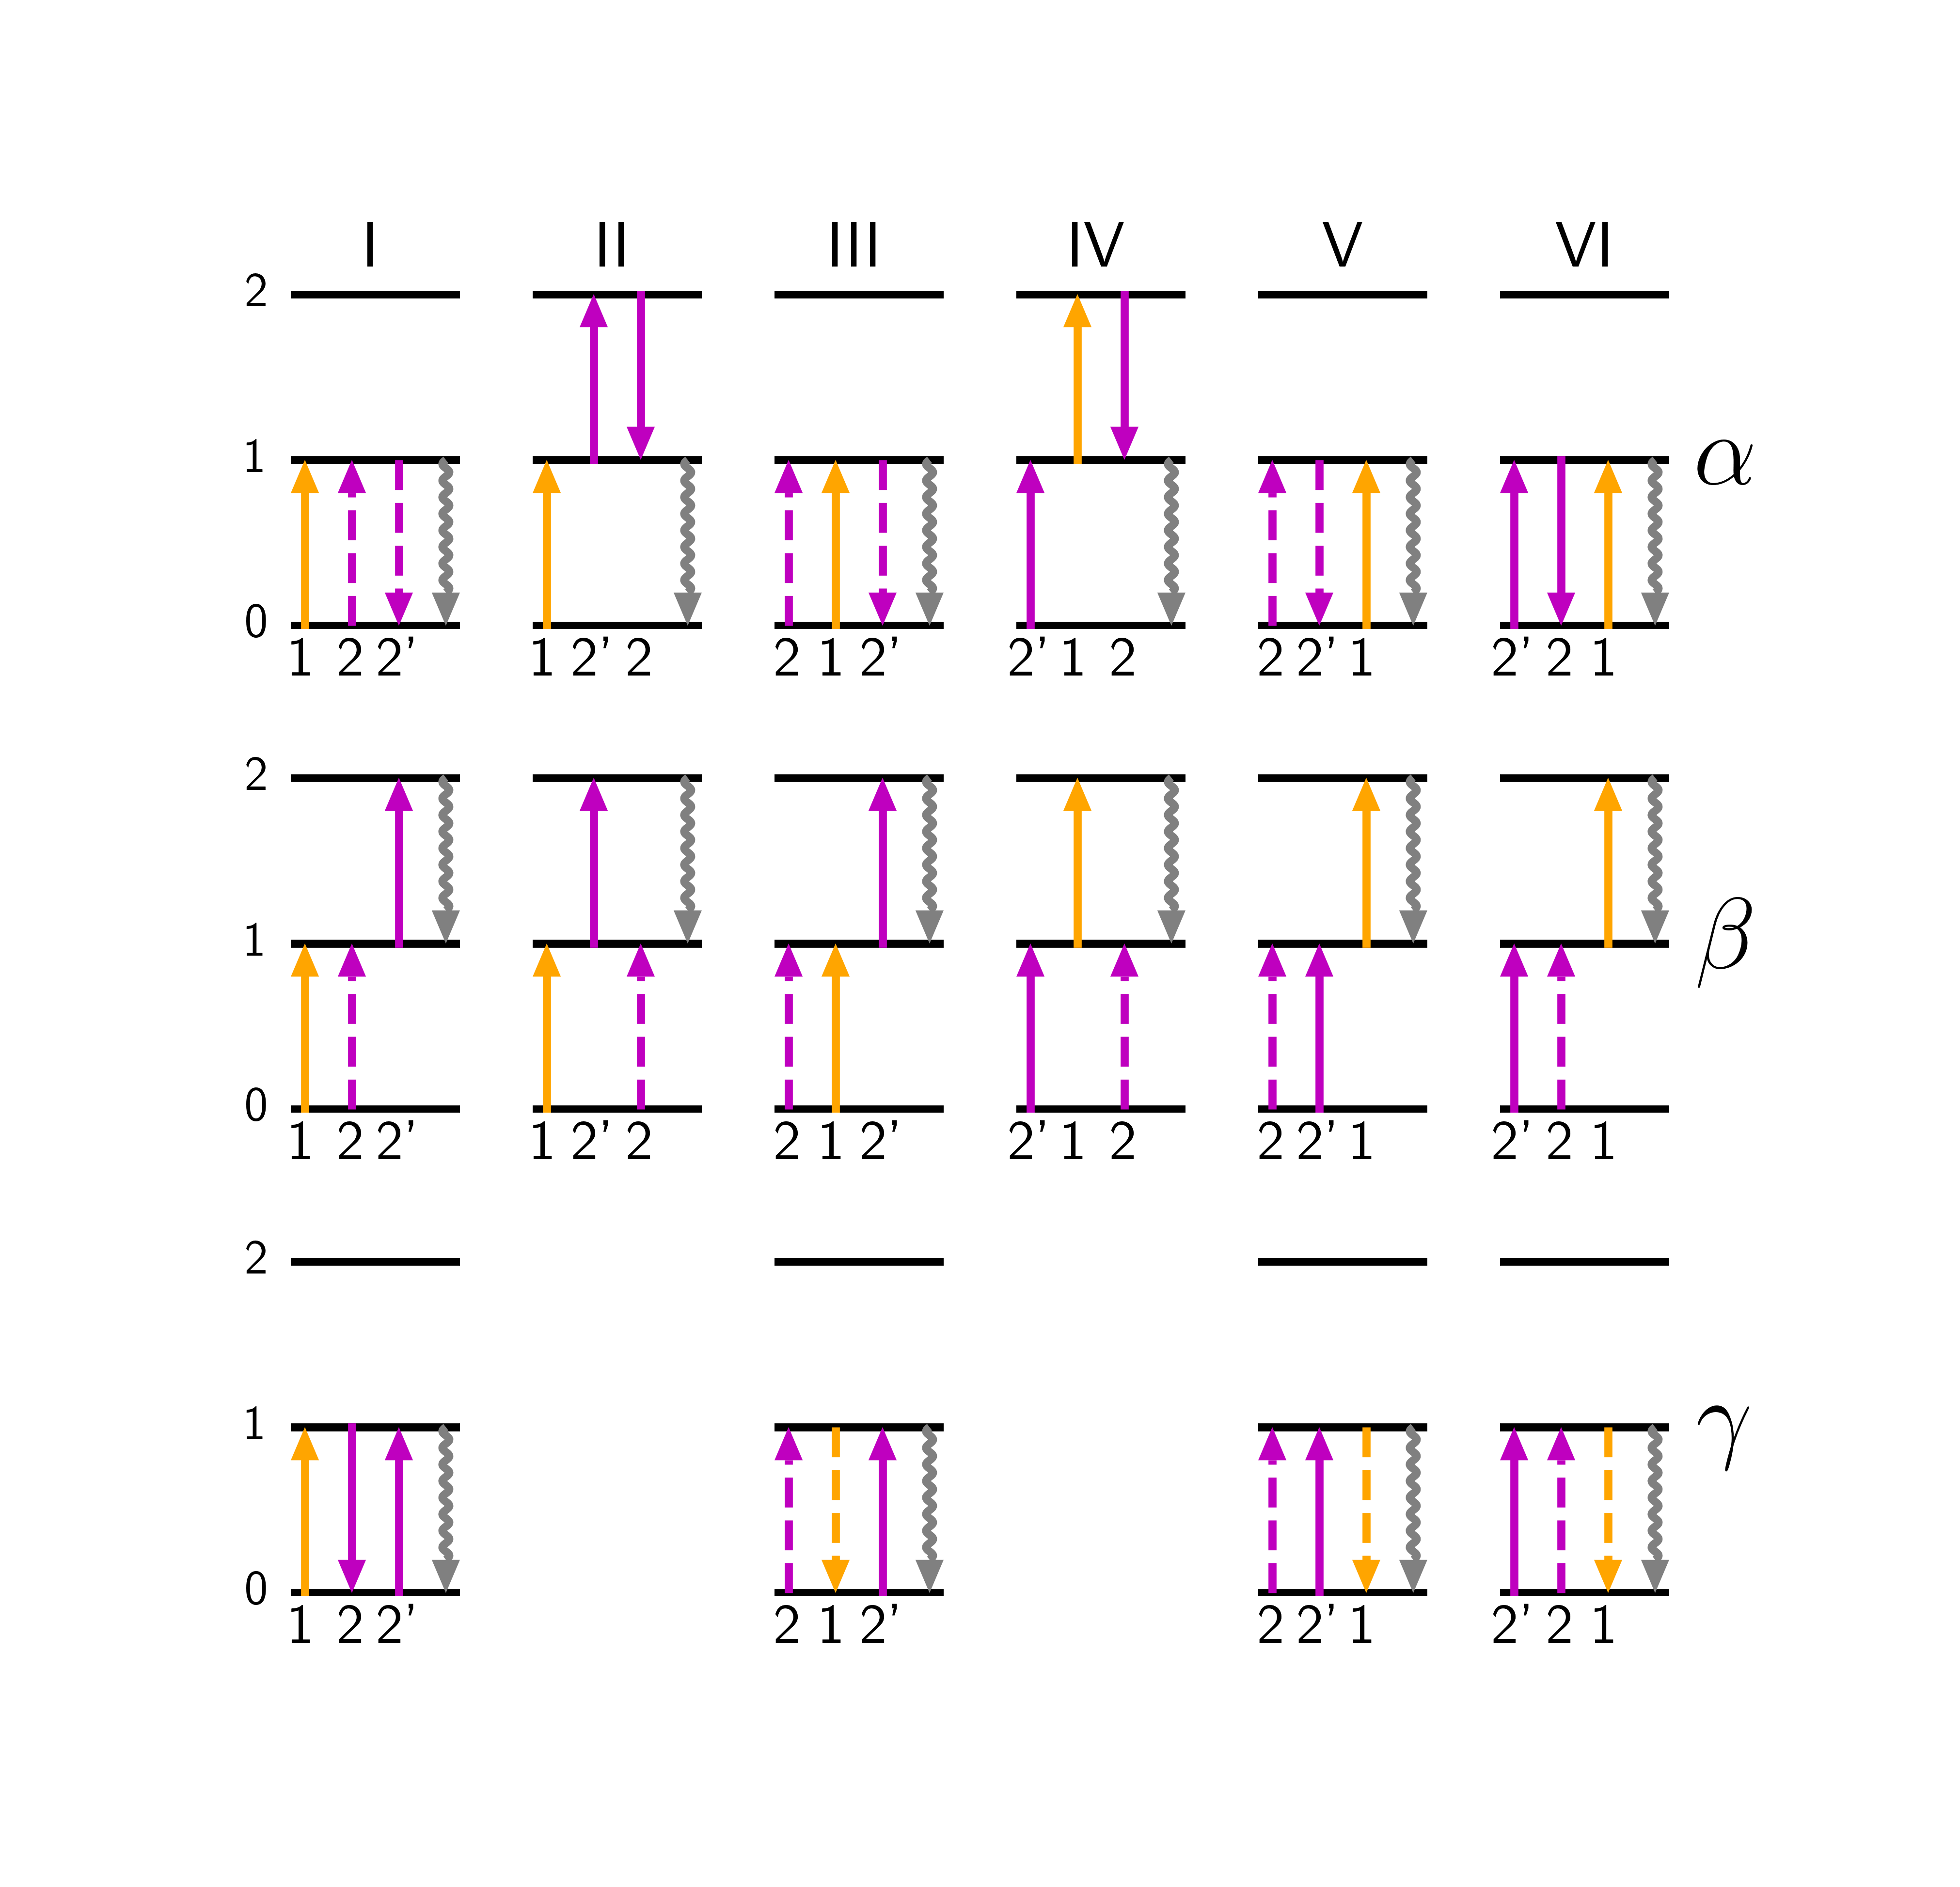
\includegraphics[height=\textheight]{WMELs}
\end{center}
\end{frame}

\begin{frame}{\textbf{Finite state automaton}}
\begin{columns}
\column{0.8\textwidth}
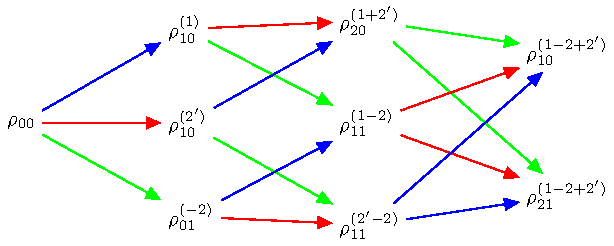
\includegraphics[width=\textwidth]{Matrix_Flow_Diagram}
\column{0.2\textwidth}
\begin{math}
\overline{\rho} \equiv
\begin{bmatrix}
\tilde{\rho}_{00} \\
\tilde{\rho}_{01}^{{-2}} \\
\tilde{\rho}_{10}^{{2^\prime}} \\
\tilde{\rho}_{10}^{{1}} \\
\tilde{\rho}_{20}^{{1+2^\prime}} \\
\tilde{\rho}_{11}^{{1-2}} \\
\tilde{\rho}_{11}^{{2^\prime-2}} \\
\tilde{\rho}_{10}^{{1-2+2^\prime}} \\
\tilde{\rho}_{21}^{{1-2+2^\prime}}
\end{bmatrix}
\end{math}
\end{columns}
\end{frame}

\begin{frame}{\textbf{Hamiltonian Matrix}}
%\begin{math}
%A_1 &\equiv& \frag{i} {2} \mu_{10}e^{-i\omega_1\tau_1)c_1(t-\tau_1)e^{i(\omega_1-\omega_{10})t} \\
%A_2 &\equiv& \frag{i} {2} \mu_{10}e^{-i\omega_2\tau_2)c_2(t-\tau_2)e^{i(\omega_2-\omega_{10})t} \\
%A_{2^\prime} &\equiv& \frag{i} {2} \mu_{10}e^{-i\omega_{2^\prime}\tau_{2^\prime})c_{2^\prime}(t-\tau_{2^\prime})e^{i(\omega_{2^\prime}-\omega_{10})t} \\
%B_1 &\equiv& \frag{i} {2} \mu_{21}e^{-i\omega_1\tau_1)c_1(t-\tau_1)e^{i(\omega_1-\omega_{21})t} \\
%B_2 &\equiv& \frag{i} {2} \mu_{21}e^{-i\omega_2\tau_2)c_2(t-\tau_2)e^{i(\omega_2-\omega_{21})t} \\
%B_{2^\prime} &\equiv& \frag{i} {2} \mu_{21}e^{-i\omega_{2^\prime}\tau_{2^\prime})c_1(t-\tau_{2^\prime})e^{i(\omega_{2^\prime}-\omega_{21})t} \\
\begin{math}
\overline{\overline{Q}} \equiv
\begin{bmatrix}
	0 & 0 & 0 & 0 & 0 & 0 & 0 & 0 & 0 \\
	-A_2 & -\Gamma_{10} & 0 & 0 & 0 & 0 & 0 & 0 & 0 \\
	A_{2^\prime} & 0 & -\Gamma_{10} & 0 & 0 & 0 & 0 & 0 & 0 \\
	A_1 & 0 & 0 & -\Gamma_{10} & 0 & 0 & 0 & 0 & 0 \\
	0 & 0 & B_1 & B_{2^\prime} & -\Gamma_{20} & 0 & 0 & 0 & 0 \\
	0 & A_1 & 0 & -A_2 & 0 & -\Gamma_{11} & 0 & 0 & 0 \\
	0 & A_{2^\prime} & -A_2 & 0 & 0 & 0 & -\Gamma_{11} & 0 & 0 \\
	0 & 0 & 0 & 0 & B_2 & -2A_{2^\prime} & -2A_1 & -\Gamma_{10} & 0 \\
	0 & 0 & 0 & 0 & -A_2 & B_{2^\prime} & B_1 & 0 & -\Gamma_{21}
\end{bmatrix}
\end{math}
\end{frame}


\section{\texttt{NISE}}

\begin{frame}{\texttt{NISE}}
	Here is some text
    %TODO text on NISE
\end{frame}

\section{\textbf{Algorithmic Improvements}}

\begin{frame}{\textbf{Algorithmic Improvements}}
	Here is some text
    %TODO text on improvements
\end{frame}

\begin{frame}{\textbf{Profile trace of \texttt{NISE}}}
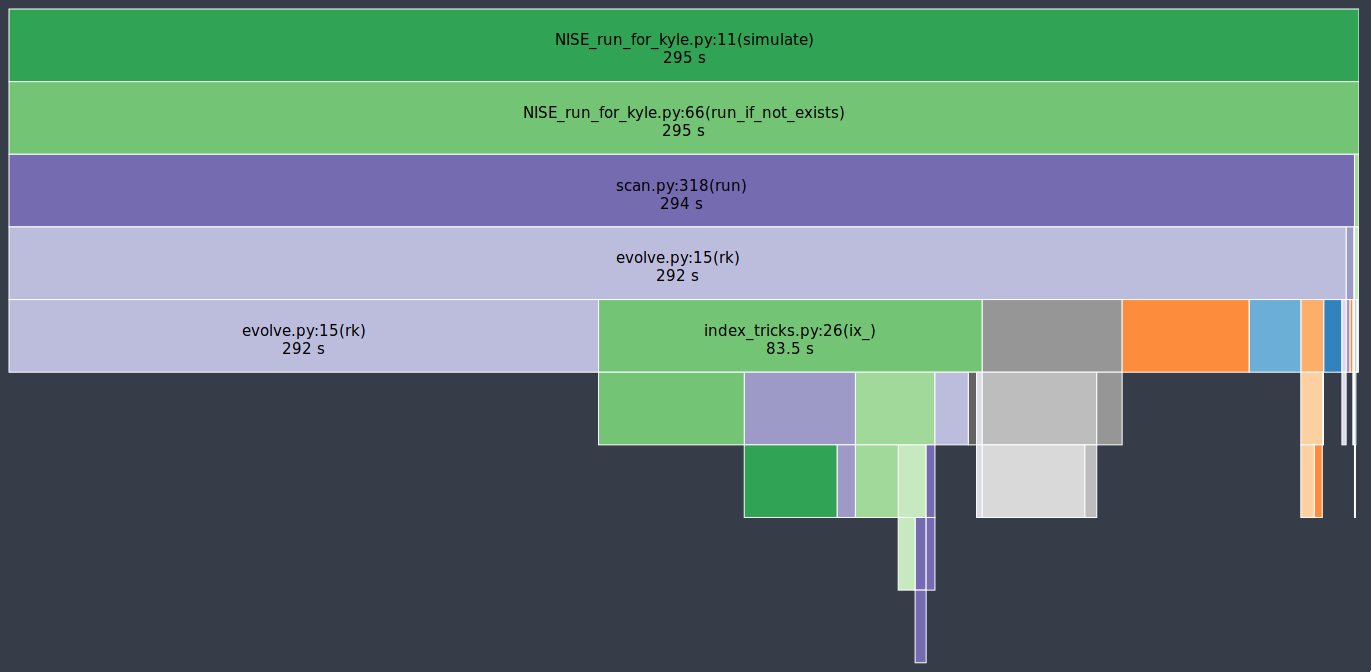
\includegraphics[width=\textwidth]{NISE_prof}
	Here is some text
    %TODO include image
\end{frame}

\begin{frame}{\textbf{Profile trace of \texttt{WrightSim}}}
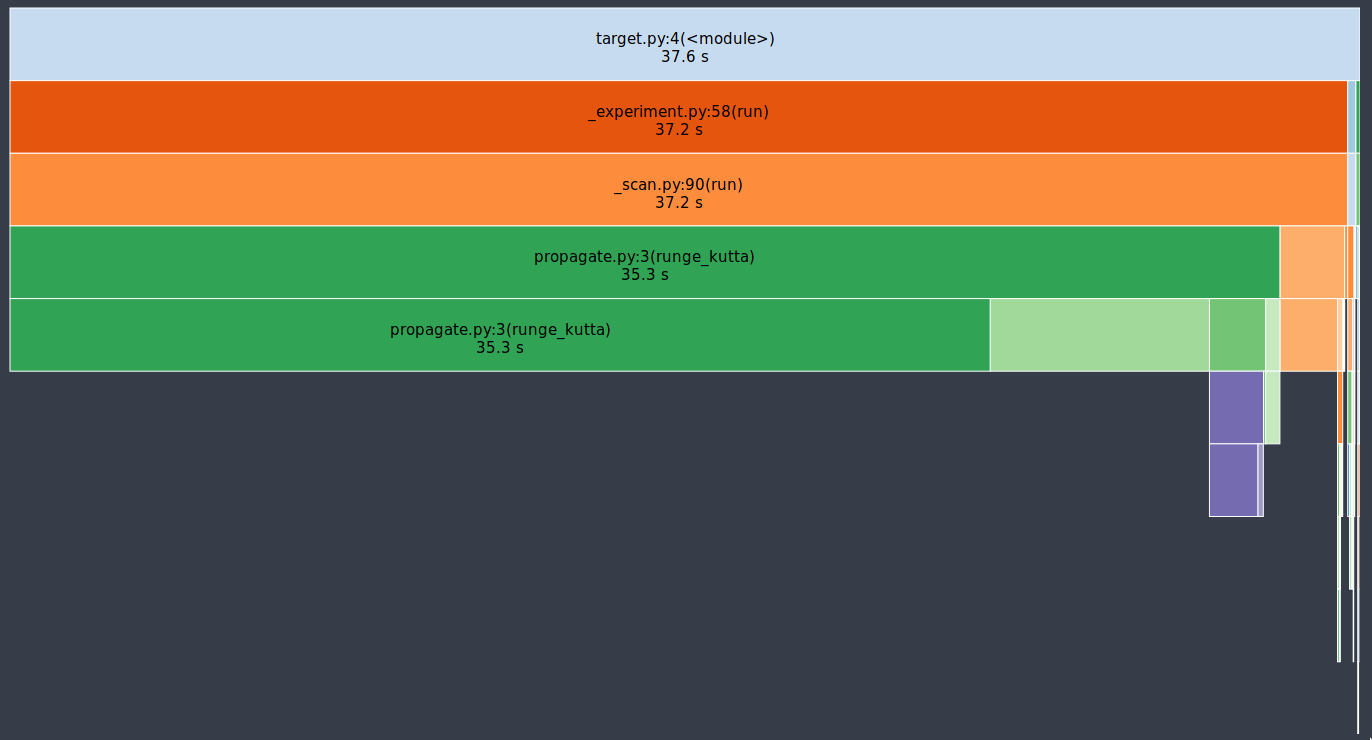
\includegraphics[width=\textwidth]{WrightSim_prof}
	Here is some text
    %TODO include image
\end{frame}

\section{\textbf{Parallel Implementations}}

\begin{frame}{\textbf{Parallel Implementations}}
	Here is some text
    %TODO text
\end{frame}

\subsection{Scaling Analysis}
\begin{frame}{\textbf{Scaling Analysis}}
\begin{center}
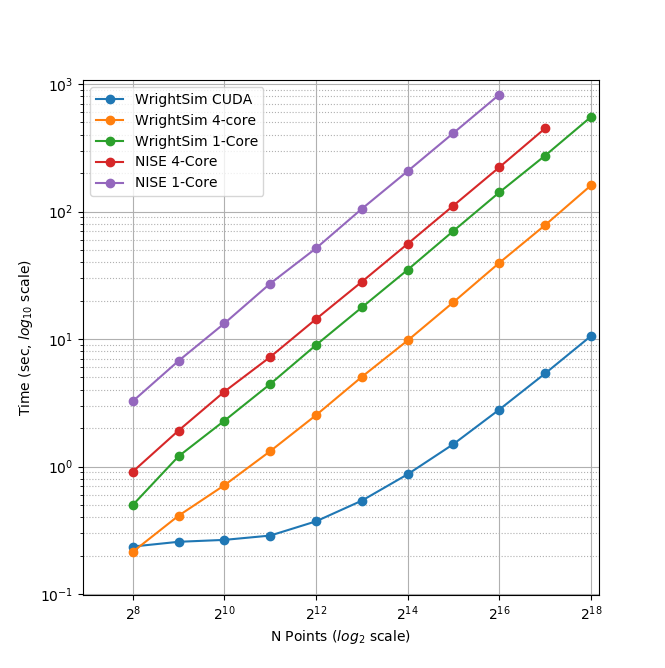
\includegraphics[height=0.8\textheight]{Scaling}
\end{center}
\end{frame}

\subsection{Limitations}

\begin{frame}{\textbf{Limitations}}
	Here is some text
    %TODO text
\end{frame}


\section{\textbf{Future Work}}

\subsection{Features}

\subsection{Usability}

\subsection{Algorithmic Improvements}

\section{\textbf{Conclusions}}

\subsection{Acknowledgements}

\section{\textbf{References}}










\end{document}
